\section{Comparison Sources and Measurement Boundaries}

Table~\ref{tab:comparison_sources} distinguishes official implementations from study-specific controls. TreePIR's Appendix J discusses sparse Merkle trees~\cite{treepir}. Figure~\ref{fig:toy_comparison} illustrates deletion and recoloring with a constructed example; the external comparison executes official TreePIR code.

\begin{figure*}[t]
\centering
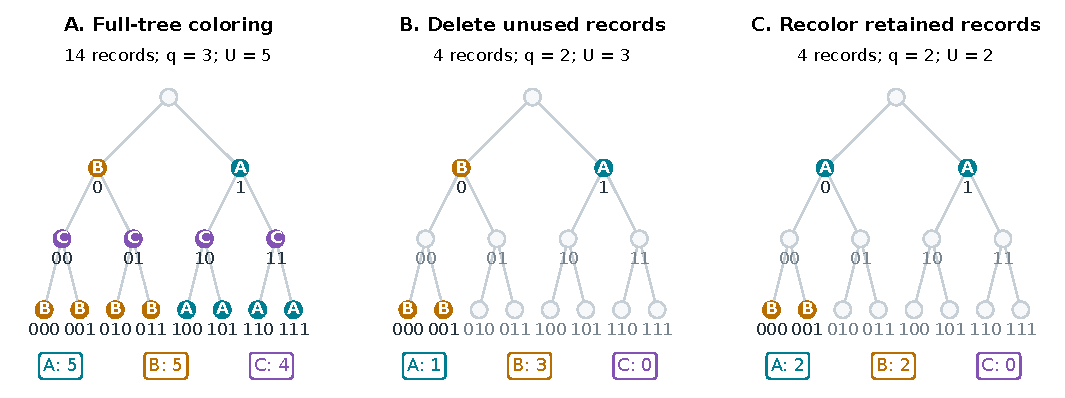
\includegraphics[width=\textwidth]{figures/supervisor_pruning_comparison.pdf}
\caption{Deletion and interval recoloring of a height-3 tree. The verified full-tree coloring is author-constructed, with 14 nonroot records, loads $(5,5,4)$, and distinct colors within each proof. Occupied slots $\{000,001,100\}$ retain four records, $\{d(0),d(1),d(000),d(001)\}$, with inherited loads $(1,3,0)$. Gray nodes are omitted, possibly nonempty records. Deleting the empty color gives $q=2$ in panel B; recoloring gives loads $(2,2)$ and capacity two instead of three, without further reducing queries. Target $000$ recovers $[d(001),\Delta_1,d(1)]$; target $100$ recovers $[\Delta_0,\Delta_1,d(0)]$ with one dummy slot. This example does not execute TreePIR or measure timing.}
\label{fig:toy_comparison}
\end{figure*}

\begin{table}[t]
\centering\small
\caption{Implementations and comparison roles.}
\label{tab:comparison_sources}
\begin{tabular}{@{}p{.27\linewidth}p{.68\linewidth}@{}}
\toprule
Method/source & Executed role\\
\midrule
TreePIR~\cite{treepir} & Original CSA/SubCSA on common complete trees.\\
VBPIR~\cite{vectorbatchpir} & Original computation core, distributed in the TreePIR repository; proof adapter specified above.\\
SimplePIR~\cite{simplepir} & Official PIR backend with the record representations specified for each experiment.\\
Nonempty-depth & Our depth partition after removing globally empty levels; not TreePIR coloring.\\
Flat-active & Our single active-record database; $m$ queries reuse its setup.\\
PBC-routed~\cite{sealpir} & Earlier PBC-based control: our three-choice placement and complete matching on SimplePIR; not native SealPIR.\\
FF, Hybrid, AB & Internal coloring controls; AB in all PIR measurements uses the original Hungarian implementation.\\
OPT witness & Separate certified Fuel layout; not a recoloring-prototype output.\\
Full-cache & All active digests and public directory; no online request.\\
\bottomrule
\end{tabular}
\end{table}

\subsection{Earlier complete-tree component validation}

The earlier comparison uses TreePIR commit \texttt{930063c5aefc441244abb4890fdf35383f3aa956}, with unchanged \texttt{CSA.java} coloring and \texttt{SubCSA.java} indexing. The original sibling swap stores the digest at node $v$ at position $v\mathbin{\mathrm{xor}}1$. The manifest pins source hashes. All 1040 leaf indices match official bucket positions; all 3120 proofs across three layouts verify before timing.

The earlier common-backend SimplePIR experiment measures 432 proofs in 18 fresh processes with paired targets and shuffled method order. Means, sample SDs, and paired intervals use three process means. Setup includes database loading and initialization, excluding layout construction. Backend wall time includes chunk retrieval and reassembly, excluding indexing, root verification, serialization, and transport. Hint plus expanded $A$ counts payload; isolated client RSS and complete-service latency are unmeasured.

The earlier VBPIR component experiment retains the original Query/Answer/Recover timers. An external adapter checks recovered siblings against the pinned root outside those timers. The C++17 build uses SEAL 4.3.2 and the original BFV parameters: degree 8192, coefficient-bit sizes $(42,58,58,60)$, 28-bit plaintexts, and first dimension 64. Both height-10 layouts have capacity 205, rounded to a $64\times4$ record grid. Build and input-path adaptations are recorded in the artifact.

\begin{table*}[t]
\centering\small
\caption{Official VBPIR core~\cite{vectorbatchpir} with portability changes and an external root-verification adapter, on the common height-10 tree. AB is ours. Times are descriptive means over ten paired targets in one process per layout, using the original C++ timing boundaries and fresh client/server objects per target. No confidence interval is estimated. Estimated query/answer sizes are the original program's serialization-size estimates, not measured wire traffic, and are not directly comparable with SimplePIR matrix bytes or TCP application bytes.}
\label{tab:official-vbpir-components}
\setlength{\tabcolsep}{8pt}
\begin{tabular}{lrrrrr}
\toprule
Layout & Query (ms) & Answer (ms) & Recover (ms) & Est. query (KiB) & Est. answer (KiB)\\
\midrule
TreePIR CSA~\cite{treepir} & 6.761 & 338.488 & 1.263 & 385 & 257\\
AB & 7.206 & 338.839 & 1.211 & 385 & 257\\
\bottomrule
\end{tabular}
\par\smallskip
\begin{minipage}{.97\textwidth}\small
Initialization: N/A, original setup is untimed. Full client state and isolated client RSS: N/A, unmeasured in this combined process. Actual wire bytes and full-service E2E: N/A, no transport and verification is outside the timers. The original estimates use query \texttt{save\_size()/2} and answer \texttt{save\_size()}, then integer division by 1024. All 20 output proofs pass independent root verification and corruption rejection.
\end{minipage}
\end{table*}


\subsection{Sparse inputs and functional checks}
\label{sec:workload-evidence}

Table~\ref{tab:workload_sources} lists six inputs: Polygon RPC samples~\cite{polygonzkevm}, ZKsync RPC samples~\cite{zksyncdocs}, and Fuel conformance vectors~\cite{fuelsmtgen}. Deduplication precedes coordinate mapping; values and roots define experimental SMTs rather than native chain state. The CT mirror uses 512 public log entries~\cite{ctlogsample}.

\begin{table*}[t]
\centering\small
\caption{Sparse input provenance. $n$ is the number of distinct occupied keys; prefixes are collision-free at both tested coordinate heights. Paths are relative to \texttt{datasets/}.}
\label{tab:workload_sources}
\begin{tabular}{@{}lrp{.56\textwidth}l@{}}
\toprule
Workload & $n$ & Input CSV & Coordinate\\
\midrule
Fuel & 100 & \path{fuel_smt_test_workload.csv} & Hex prefix\\
Polygon recent & 384 & \path{polygon_zkevm_account_leaf_workload.csv} & SHA-256 prefix\\
ZKsync sample & 956 & \path{zksync_era_account_leaf_workload_sample.csv} & SHA-256 prefix\\
Polygon multi & 1348 & \path{polygon_zkevm_account_leaf_workload_multiwindow.csv} & SHA-256 prefix\\
Polygon broad & 7040 & \path{polygon_zkevm_account_leaf_workload_broad_multiwindow.csv} & SHA-256 prefix\\
ZKsync broad & 7740 & \path{zksync_era_account_leaf_workload_broad_sample.csv} & SHA-256 prefix\\
\bottomrule
\end{tabular}
\end{table*}

The six-workload suite uses five processes per method/workload, five warmups, and 100 paired targets; all 18000 proofs verify. Separate checks cover 2153 proofs across 332 layouts, all 278 occupied sets at heights 0--3 against a dense oracle, and height-128/256 boundaries. Routing covers six methods on ten trees. Matching agrees with brute force on 256 graphs and rejects a Hall failure. Wrong roots, levels, and digest flips are rejected. These are implementation checks.

\subsection{Coloring-control parameters}
\label{sec:coloring-control-protocol}

Hybrid uses \texttt{color\_proof\_nodes} in \path{scripts/run_sparse_smt_pir_backend_experiment.py}. Let $C_i$ count records of color $i$, $W_i$ sum their weights $w(v)=|I_v|$, and $\Delta_C,\Delta_W$ denote the respective maximum-minus-minimum ranges. The score is
\begin{equation}
J_{\rm H}=\frac{\Delta_C}{\max(1,\overline C)}
          +\frac{\Delta_W}{\max(1,\overline W)}.
\label{eq:hybrid-control-score}
\end{equation}
Traversal visits roots and children by descending weight. Among ancestor-available colors, it minimizes $(J_{\rm H},\Delta_C,\Delta_W,|C_i-t_i|,i)$, where $t_i=\lfloor N/m\rfloor+\mathbf{1}[i\le N\bmod m]$. Refinement selects the best proper single-node move under $(J_{\rm H},\Delta_C,\Delta_W,\max_i C_i,\max_i W_i)$, accepts strict improvements, and stops at a local optimum or 60 moves. Traversal order breaks remaining ties.

AB uses \texttt{best\_count\_profile\_balanced} in \path{scripts/run_height_sparsity_profile_balance_experiment.py}. From smallest-available ancestor coloring, it evaluates permitted subtree permutations with Hungarian assignment and accepts the best strict decrease of the sorted load vector. It stops after $R_1=20$ scans or at a local optimum. Construction is outside online timing; the manifest pins both controls and the measured driver.

\subsection{Directory, hints, and full-cache accounting}
\label{sec:setup-costs}

At the tested byte-aligned heights, serialized AB directory and complete cache sizes are
\begin{align}
M_{\rm AB}&=24N+18+8m+nh/8,\label{eq:measured-directory}\\
F_{\rm cache}&=56N+26+nh/8.\label{eq:measured-cache}
\end{align}
Both include occupied coordinates. Table~\ref{tab:setup-costs} reports directory, hint, and expanded-matrix payloads, excluding TCP framing and peak memory. KiB and MiB are binary units; the conceptual $2^{h+1}-1$ nodes are not a storage denominator.

\begin{table}[t]
\centering\small\setlength{\tabcolsep}{3pt}
\caption{AB (ours) initialization payloads under SimplePIR~\cite{simplepir} and the complete cache package for the six height-128 inputs. $A$ is the expanded public matrix; cache includes digests and its directory.}
\label{tab:setup-costs}
\begin{tabular}{@{}lrrrr@{}}
\toprule
Workload & Dir. KiB & Hint MiB & $A$ MiB & Cache KiB\\
\midrule
Fuel & 6.29 & 3.38 & 2.22 & 12.42\\
Polygon recent & 24.06 & 5.50 & 6.19 & 47.92\\
ZKsync sample & 59.82 & 9.75 & 10.16 & 119.42\\
Polygon multi & 84.33 & 12.25 & 12.25 & 168.42\\
Polygon broad & 440.10 & 31.88 & 29.75 & 879.92\\
ZKsync broad & 483.85 & 31.88 & 32.41 & 967.42\\
\bottomrule
\end{tabular}
\end{table}

Storage accounting distinguishes packed coordinates $nh/8$, active digests $32N$, and all nonempty-node digests $32S$, including unary ancestors. At height 128, $M_{\rm AB}/(nh/8)=4.001$--$4.026$ and $100M_{\rm AB}/(32S)=1.643$--$1.722\%$. Extending distinct prefixes to height 256 preserves active intervals and gives $S_{256}=S_{128}+128n$; this is structural accounting, not backend timing.

\subsection{Native long-record packing}
\label{sec:followup-packing}

Vertical 256-bit SimplePIR packing~\cite{simplepir} passes 1075 retained-record and 50 boundary checks on the CT snapshot. Near-square shapes use 4168/4828 matrix bytes per proof for First-fit/AB; one-record rows use 5504 for either layout. TCP timing is unmeasured.

With the pinned plaintext modulus $p\le991$, a 256-bit digest needs at least 26 base-$p$ entries. An uncompressed hint contains $L\times1024$ 32-bit coefficients, requiring at least
\begin{equation}
H_{\min}=26\cdot1024\cdot4=106496\ \text{bytes}.
\label{eq:native-hint-floor}
\end{equation}
Summed over nonempty independent buckets, this exceeds the active-digest payload on each of the six application-derived snapshots and the 512-entry CT snapshot used in this earlier packing study. PIR and cache share coordinate and directory terms; PIR adds bucket headers. This bound applies only to the pinned hint construction and these named snapshots. Query privacy does not imply database privacy or authorization~\cite{spirprivacy}.

\begin{table}[t]
\centering\small
\caption{Evidence directories under \texttt{examples/}. Manifests pin sources, inputs, and raw records.}
\label{tab:source_manifest}
\begin{tabular}{@{}p{.25\linewidth}p{.70\linewidth}@{}}
\toprule
Evidence & Directory\\
\midrule
Official comparison & \path{tifs_contribution_gate_20260910/external/}\\
Native VBPIR & \path{tifs_external_extension_20260911/}\\
Native SimplePIR & \path{tifs_simplepir_extension_20260911/}\\
18000 local proofs & \path{tifs_revision_20260910/verified_backend/}\\
SMT/routing tests & \path{tifs_revision_20260910/correctness/}\\
CT TCP & \path{tifs_revision_20260910/ct_application/runs_verified_evidence/}\\
Fuel TCP & \path{tifs_layout_transfer_20260910/system/}\\
Exact capacities & \path{tifs_remaining_gap_20260910/}\\
Bounded refinement & \path{tifs_sufficiency_20260910/construction/}\\
Construction scale & \path{tifs_revision_20260910/balance_repeats/}\\
\bottomrule
\end{tabular}
\end{table}

\subsection{Construction scale and censored runs}
\label{sec:construction-scale}

The sorting implementation evaluates the count-only objective in Section~\ref{sec:ab-sorting-assignment}. Candidate equivalence holds across 939 configurations and 181665 permutations; ties may change later colorings. The construction study uses Windows and Python 3.14, with three fresh processes on the same 100000-leaf uniform instance and a 20-scan budget (Table~\ref{tab:construction-scale}).

\begin{table}[t]
\centering\small\setlength{\tabcolsep}{3pt}
\caption{Construction at 100000 uniform leaves. Completed-run values are mean $\pm$ sample SD over three processes. The Hungarian runs are right-censored at 120\,s; their final 20-scan time, quality, and memory are unavailable.}
\label{tab:construction-scale}
\begin{tabular}{@{}lrr@{}}
\toprule
Metric & Sorting AB & Hungarian AB\\
\midrule
Completed runs & 3/3 & 0/3\\
Completed scans & 20 & 9--10 before stop\\
Coloring (s) & $40.984\pm4.899$ & Censored\\
Process wall (s) & $46.149\pm4.973$ & $\ge120$\\
Observed RSS (MiB) & $763.5\pm0.9$ & $655.5\pm0.5$\\
Final $U/B$ & 1.00385 & Unavailable\\
\bottomrule
\end{tabular}
\end{table}

All sorting runs finish with $U=9126$. Hungarian checkpoint ratios are 1.16687, 1.45276, and 1.45276; these and observed RSS describe execution before termination, not completed 20-scan results. Censored runs provide neither completion times nor an exact speedup. The artifact retains per-run histories and memory samples.
